\section{Polimorfismo: cos'è e perché serve}
Sebbene il processo di analisi di un dominio applicativo tenda a favorire la sua
suddivisione in una molteplicità di tipi distinti (classi, strutture, funzioni,
ecc.), la necessità di minimizzare il codice scritto spinge verso
l'identificazione di comportamenti comuni, che possano essere condivisi tra tali
tipi per unificare la struttura del codice \footnote{Ciò sta alla base del principio DRY - Don't Repeat Yourself.}



La soluzione individuata è il \textbf{polimorfismo}: capacità di associare comportamenti
comuni ad un insieme di tipi differenti, così da rendere più compatta e
razionale la struttura del codice

\section{Implementare il polimorfismo}

Linguaggi di programmazione diversi hanno introdotto vari modi per implementare
il polimorfismo:

\begin{itemize}
  \item Può basarsi sul paradigma della \textbf{programmazione generica}, dove è
        possibile formulare funzioni o strutture dati in cui uno o più tipi non sono
        specificati per nome, ma tramite simboli astratti, abilitando così la
        scrittura di codice in grado di operare con una molteplicità di tipi
  \item può sfruttare la definizione di \textbf{interfacce} comuni, che possono essere
        implementate dai singoli tipi. Questo consente di fare riferimento
        all'interfaccia invece che al tipo concreto
  \item Nei linguaggi che implementano il concetto di \textbf{ereditarietà}, il
        polimorfismo si può realizzare derivando più classi concrete da una
        super-classe in cui è definito il comportamento comune
\end{itemize}

\section{Il polimorfismo in Rust si basa sui tratti}
In Rust un tratto, \textit{trait}, descrive un comportamento:

\begin{itemize}
  \item Un valore può essere stampato
  \item Due valori omogenei possono essere confrontati tra loro
  \item Il contenuto di una collezione può essere esaminato un elemento alla volta
\end{itemize}

Un tipo, predefinito o definito dall'utente, può implementare zero, uno o più
tratti acquisendo la capacità di eseguire i corrispondenti comportamenti e
rendendo nota questa capacità al compilatore che ne potrà usufruire per generare
e ottimizzare il codice.

I tratti in Rust costituiscono l'equivalente concettuale delle interfacce di
Java e C\#, infatti definiscono un \textbf{insieme di metodi}, eventualmente associando loro un’implementazione di
default.

\paragraph{Esempio}
I tratti abilitano costrutti reali:
\begin{itemize}
  \item \mintinline{rust}|println!("{}", x)| possibile se il tipo di \texttt{x} implementa il tratto \texttt{Display}
  \item \mintinline{rust}|println!("{:?}", x)| possibile se il tipo di \texttt{x} implementa il tratto \texttt{Debug}
  \item \mintinline{rust}|for x in v {...}| possibile se il tipo di \texttt{x} implementa il tratto \texttt{IntoIterator}
  \item \mintinline{rust}|a == b| possibile se il tipo di \texttt{a} e \texttt{b} implementa il tratto \texttt{PartialEq}
\end{itemize}

Una porzione significativa della sintassi di Rust è basata sul concetto di
tratto e su un insieme di tratti che fanno parte della libreria standard.
Oltre a questi tratti predefiniti, possono essere affiancati tratti definiti dall'utente.


\subsection{Definire un tratto}


\begin{minted}[breaklines]{rust}
trait Validatable {
  fn validate(&self) -> bool;
}  
\end{minted}

Un tratto definisce un \textbf{comportamento}, non un tipo concreto.
In questo caso, stiamo dicendo che i tipi che implementeranno il tratto
\textit{Validatable} dovranno avere un meccanismo - la funzione \mintinline{rust}|validate(...)| - volto
a stabilire se il loro contenuto è valido, secondo una qualche interpretazione
legata al dominio che modellano, o meno.

\subsection{Implementare un tratto per un dato tipo}

\begin{center}
  \begin{minipage}{0.45\linewidth}
    Il costrutto \mintinline{rust}|impl <trait> for <type> { ... }| e specifica, al
    tempo stesso, l'implementazione dei metodi corrispondenti.

    Tale costrutto è separato da quello relativo all'implementazione dei
    metodi peculiari al tipo: \mintinline{rust}|impl <type> { ... }|
  \end{minipage}%
  \hfill
  \begin{minipage}{0.45\linewidth}
    \begin{minted}[breaklines]{rust}
struct User {
  name: String,
  age: u8;
}
impl Validatable for User {
  fn validate(&self) -> bool {
  self.name.trim().len() > 0 &&
    self.age >= 18
  }
}

impl User { /* metodi di User */ }
\end{minted}
  \end{minipage}
\end{center}

\subsection{Un tratto può essere implementato da molti tipi}

\begin{center}
  \begin{minipage}{0.45\linewidth}
    Lo stesso comportamento viene realizzato in modi differenti in base al tipo
    specifico, ciò che resta comune è l'insieme dei metodi offerti dal tratto e la
    loro firma.

  \end{minipage}%
  \hfill
  \begin{minipage}{0.45\linewidth}
    \begin{minted}[breaklines]{rust}
struct Order {
  total: f64,
  quantity: u32
}
impl Validatable for Order {
  fn validate(&self) -> bool {
    self.total > 0 &&
    self.quantity > 0
  }
}
impl Order { /* ... */ }
\end{minted}
  \end{minipage}
\end{center}


\subsection{Un tratto può essere implementato dai tipi esistenti}

\begin{center}
  \begin{minipage}{0.45\linewidth}
    È lecito che un tipo esistente implementi un tratto definito dall'utente.


    Rust impone regole precise su dove sia lecito scrivere un'implementazione,
    per evitare conflitti
  \end{minipage}%
  \hfill
  \begin{minipage}{0.45\linewidth}
    \begin{minted}[breaklines]{rust}
impl Validatable for String {
  fn validate(&self) -> bool {
    self.trim().len() > 0
  }
}
impl Validatable for i32 {
  fn validate(&self) -> bool {
    *self > 0
  }
}
\end{minted}
  \end{minipage}
\end{center}


\subsection{Invocare i metodi di un tratto}


\begin{center}
  \begin{minipage}{0.45\linewidth}
    Se il tipo concreto di un valore è noto,
    chiamare i metodi di un tratto non ha
    differenze rispetto a chiamare i metodi
    specifici del tipo.

    Non solo sul piano sintattico, ma anche
    su quello del codice generato.

    La chiamata viene risolta staticamente
    e non introduce penalizzazioni
  \end{minipage}%
  \hfill
  \begin{minipage}{0.45\linewidth}
    \begin{minted}[breaklines]{rust}
let u: User = User {
  name: "Mario".to_string(),
  age: 32
};
let o: Order = Order {
  total: 1200.0,
  quantity: 8
};
u.validate();
o.validate();
\end{minted}
  \end{minipage}
\end{center}

\section{I tratti come vincoli}


\begin{center}
  \begin{minted}[breaklines]{rust}
                            fn check<T: Validatable>(item: &T) {
                              println!("{}", item.validate());
                            }
\end{minted}
\end{center}

Questa funzione accetta come parametro solo valori il cui tipo implementa il
tratto \textit{Validatable}.

Tentativi di passare a questa funzione tipi privi del tratto danno origine ad un
errore in fase di compilazione.

La conoscenza specifica del tipo, rappresentato dalla meta-variabile T, permette
al compilatore di ottimizzare il codice generato


\subsection{Due modi di usare un tratto}

\begin{center}
  \begin{minipage}[t]{0.47\linewidth}
    Come vincolo su un tipo generico. Quando il tipo concreto di un valore è noto
    al compilatore, la chiamata viene risolta staticamente. Questo è il caso più
    comune

    \begin{minted}[breaklines]{rust}    
fn process1<T: Validatable>(x: &T) {
  println!("{}", x.validate());
}
    \end{minted}

  \end{minipage}
  \hfill
  \begin{minipage}[t]{0.47\linewidth}
    Come oggetto-tratto con invocazione dinamica.
    Se il tipo concreto è nascosto dietro l'interfaccia, la scelta del
    metodo avviene in fase di esecuzione. La parola chiave dyn indica un
    oggetto-tratto, ovvero ad un puntatore di cui si sa solo che punta ad un
    dato che implementa il tratto

    \begin{minted}[breaklines]{rust}
fn process2(x: &dyn Validatable) {
  println!("{}", x.validate());
}
    \end{minted}

  \end{minipage}
\end{center}

\section{Invocazione dinamica}

\begin{center}
  \begin{minipage}{0.45\linewidth}
    La parola chiave dyn segnala l'uso del tratto come oggetto-tratto.
    I metodi vengono risolti in fase di esecuzione.
    Questo mette in evidenza al programmatore che il programma dovrà utilizzare il meccanismo di invocazione dinamica (dynamic dispatch)
  \end{minipage}%
  \hfill
  \begin{minipage}{0.45\linewidth}
    \begin{minted}[breaklines]{rust}  
fn process(x: &dyn Validatable) {
  println!("{}", x.validate());
}
fn main() {
  let u = User { … };
  let o = Order { … };
  process(&u);
  process(&o);
}
\end{minted}
  \end{minipage}
\end{center}

\section{Oggetti-tratto}

\begin{center}
  \begin{minipage}{0.6\linewidth}
    I riferimenti/puntatori ai tipi tratto vengono detti oggetti-tratto.

    Possono essere condivisi o mutabili e devono rispettare le regole
    dell'esistenza in vita del valore a cui fanno riferimento.


    Gli oggetti-tratto vengono implementati tramite fat pointer.
  \end{minipage}%
  \hfill
  \begin{minipage}{0.35\linewidth}
    \centering
    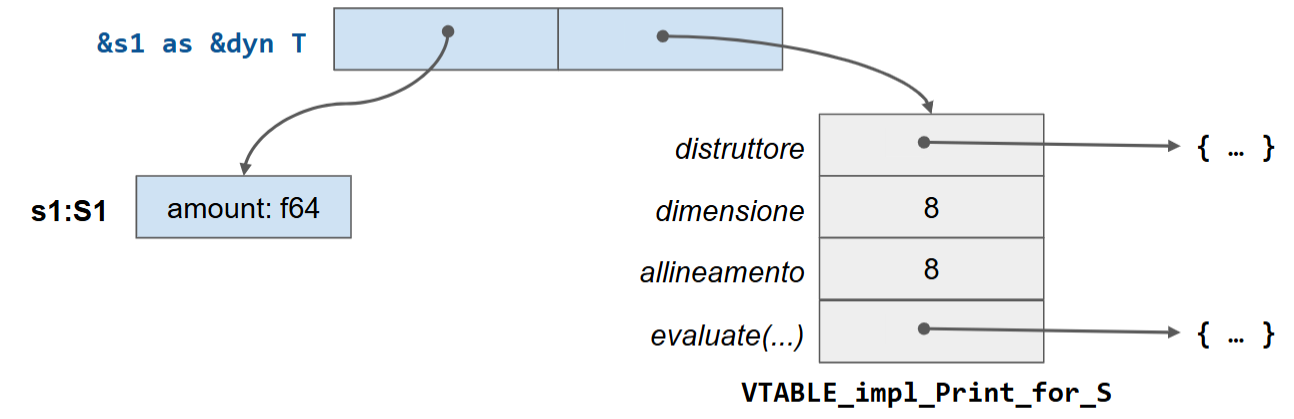
\includegraphics[width=\linewidth]{content/API_Programming/images/2026-03-24-12-19-24.png}
  \end{minipage}
\end{center}

\section{Vincoli degli oggetti-tratto}

Non tutti i tratti possono essere referenziati dinamicamente. Il compilatore
deve, infatti, essere in grado di costruire la vtable associata al tratto.

Un tratto è compatibile con l'invocazione dinamica se i suoi metodi soddisfano i
seguenti vincoli:

\begin{itemize}
  \item Operano su \verb|&self| o \verb|&mut self| sono metodi a livello istanza che non
        consumano il ricevitore
  \item Non restituiscono \verb|Self|
  \item Non contengono parametri generici
\end{itemize}

\section{Tratti con implementazioni di default}
Nella definizione di un tratto è lecito indicare, per una data funzione,
un'implementazione di default.

Le funzioni che implementano il tratto saranno libere di adottarla o potranno
sovrascriverla con altro codice, purché venga rispettata la firma delle funzione,
tipo dei parametri e del valore di ritorno.


\begin{center}
  \begin{minipage}{0.47\linewidth}
    \begin{minted}[breaklines]{rust}    
    trait T4 {
      fn f() { println!("default"); }
    }
    \end{minted}
    \vfill
    \begin{minted}[breaklines]{rust}    
    struct OtherType;
    impl T4 for OtherType {
      fn f() { println!("Other"); }
    }
    \end{minted}

  \end{minipage}
  \hfill
  \begin{minipage}{0.47\linewidth}
    \begin{minted}[breaklines]{rust}    
    struct SomeType;
    impl T4 for SomeType { }
    //uso dell'implementazione di default
    \end{minted}
    \vfill
    \begin{minted}[breaklines]{rust}    
    fn main() {
      SomeType::f(); // default
      OtherType::f(); // Other
    }
    \end{minted}

  \end{minipage}
\end{center}

\section{Tipi e tratti}



\begin{center}
  \begin{minipage}{0.6\linewidth}

    Poiché tipi diversi possono implementare tratti comuni, si viene a creare una
    forma di ``parentela'' alquanto articolata tra tipi.

    Rust introduce una ventina di tratti predefiniti, cui il compilatore associa un
    particolare significato, e permette al programmatore di aggiungerne altri a
    piacere, al fine di estendere tale comportamento.
  \end{minipage}%
  \hfill
  \begin{minipage}{0.35\linewidth}
    \centering
    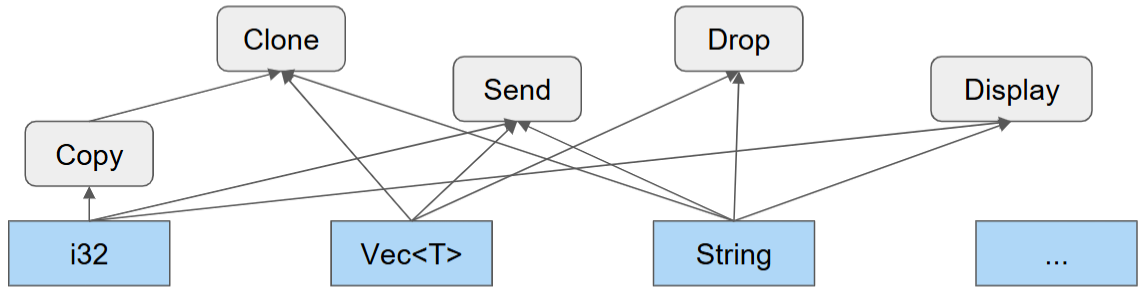
\includegraphics[width=\linewidth]{content/API_Programming/images/2026-03-24-12-30-17.png}
  \end{minipage}
\end{center}

\begin{tcolorbox}
  \textbf{Nota:} In Rust i tratti non classificano i tipi in una gerarchia
  unica, ma descrivono proprietà e comportamenti trasversali
\end{tcolorbox}

\section{Programmazione generica}
Notazione che permette di scrivere funzioni, strutture dati e tratti che
utilizzano diversi tipi di dati senza duplicare il codice, tramite parametri
generici.
Consente di mantenere il codice flessibile, riutilizzabile e sicuro
grazie al controllo dei tipi in fase di compilazione.

In Rust la programmazione generica si combina naturalmente con i tratti, che
permettono di vincolare i tipi generici a comportamenti specifici.

\begin{minted}[breaklines]{rust}
              fn first<T>(slice: &[T]) -> Option<&T> {
                slice.get(0)
              }
\end{minted}

\begin{tcolorbox}
  \textbf{Nota: } T parametro generico che rappresenta un tipo
\end{tcolorbox}

\section{Funzioni generiche}

\begin{center}
  \begin{minipage}{0.65\linewidth}
    Si può definire una funzione in modo che operi su un tipo di dato non ancora
    precisato.
    Rappresentato da un segnaposto racchiuso tra < e >. \verb|T| è generico ma non
    arbitrario: deve implementare il tratto \verb|PartialOrd|

  \end{minipage}%
  \hfill
  \begin{minipage}{0.3\linewidth}
    \begin{minted}[breaklines]{rust}
fn max<T>(t1: T, t2: T) -> T
where T: PartialOrd {
  if t1 > t2 { t1 }
  else { t2 }
}
\end{minted}
  \end{minipage}
\end{center}

\section{Dall'astrazione al codice concreto}

Al momento della chiamata, il compilatore:

\begin{itemize}
  \item Deduce il tipo di \verb|T|
  \item Controlla che soddisfi tutti i vincoli cui è soggetto
  \item Genera una versione specializzata della funzione per quel tipo
\end{itemize}

Se la funzione generica viene invocata in più punti del programma con tipi
diversi. Il compilatore genererà tante versioni della funzione quanti sono i
tipi con cui viene utilizzata.

Questo processo è detto \textbf{monomorfizzazione}.

\section{Tipi generici}

Si possono usare costrutti generici anche per definire un tipo composto, struct,
tupla, enum, basato su parti variabili.

Ciascuna meta-variabile può essere soggetta ad eventuali restrizioni, indicate
come l'insieme dei tratti che deve implementare e/o come il tempo di vita che
deve garantire.


Se una struttura generica implementa dei metodi, i nomi delle meta-variabili ed
i vincoli cui sono soggette vengono ripetuti nel blocco \mintinline{rust}{impl}.



\begin{center}
  \begin{minipage}{0.47\linewidth}
    \begin{minted}[breaklines]{rust}    
        struct MyStruct<T>
          where T: SomeTrait {
          value: T
        }
    \end{minted}

  \end{minipage}
  \hfill
  \begin{minipage}{0.47\linewidth}
    \begin{minted}[breaklines]{rust}
      impl<T> MyStruct<T>
        where T: SomeTrait {
        fn process(&self) { /.../ }
      }
    \end{minted}

  \end{minipage}
\end{center}


\section{Sintassi dei tipi generici}

Rust offre due modi per specificare la sintassi dei vincoli sui tipi generici:

\begin{itemize}
  \item Una versione compatta \verb|<T: SomeTrait>|
  \item La versione estesa \verb|<T> ... where T: SomeTrait|
\end{itemize}

In entrambi i casi, se è necessario indicare che il tipo deve implementare più tratti,
questi possono essere combinati con il segno +.


\begin{center}
  \begin{minipage}{0.47\linewidth}
    \begin{minted}[breaklines]{rust}    
        struct MyStruct<T>
          where T: SomeTrait {
          value: T
        }
    \end{minted}

  \end{minipage}
  \hfill
  \begin{minipage}{0.47\linewidth}
    \begin{minted}[breaklines]{rust}
        impl<T> MyStruct<T>
          where T: SomeTrait {
          fn process(&self) { /.../ }
        }
    \end{minted}

  \end{minipage}
\end{center}

\section{Tratti con tipi associati}

Un tratto può associare uno o più tipi al comportamento che descrive.
Il tipo associato fa parte della definizione del tratto. Chi implementa il
tratto deve specificarne il valore concreto.
Questo è utile quando un comportamento dipende anche da un tipo collegato.

\begin{center}
  \begin{minipage}{0.47\linewidth}
    \begin{minted}[breaklines]{rust}
        trait Container {
          type Item;
        
          fn get(&self) -> &Self::Item;
        }
    \end{minted}

  \end{minipage}
  \hfill
  \begin{minipage}{0.47\linewidth}
    \begin{minted}[breaklines]{rust}
        struct IntBox(i32);
        
        impl Container for IntBox {
          type Item = i32;
        
          fn get(&self) -> &Self::Item {
            &self.0
          }
        }
    \end{minted}
  \end{minipage}
\end{center}

\begin{tcolorbox}
  \textbf{Nota:} Un tratto non descrive solo metodi, ma anche tipi associati
  al comportamento
\end{tcolorbox}

\section{Tipi associati e generics}
I tipi associati possono dipendere da un parametro generico del tipo che
implementa il tratto:

\begin{itemize}
  \item Il tratto definisce il tipo associato
  \item L'implementazione concreta ne specifica il valore
  \item Se il tipo che implementa il tratto è generico, anche il tipo associato può dipendere da quel parametro
\end{itemize}

\begin{center}
  \begin{minipage}{0.47\linewidth}
    \begin{minted}[breaklines]{rust}
        trait Container {
          type Item;
        
          fn get(&self) -> &Self::Item;
        }
    \end{minted}

  \end{minipage}
  \hfill
  \begin{minipage}{0.47\linewidth}
    \begin{minted}[breaklines]{rust}
        struct Boxed<T>(T);
        
        impl<T> Container for Boxed<T> {
          type Item = T;
        
          fn get(&self) -> &Self::Item {
            &self.0
          }
        }
    \end{minted}
  \end{minipage}
\end{center}

\begin{tcolorbox}
  \textbf{Note:} Il tipo associato in questo caso coincide con il parametro
  generico T
\end{tcolorbox}


\section{Super-tratti}
Un tratto può richiedere che chi lo implementa implementi anche un altro tratto

Se \verb|TrattoB: TrattoA|, allora ogni tipo che implementa \verb|TrattoB| deve implementare anche \verb|TrattoA|.
Questo permette di costruire tratti più specifici a partire da tratti più generali



\begin{center}
  \begin{minipage}{0.47\linewidth}
    \begin{minted}[breaklines]{rust}
        trait Printable{
          fn print(&self);
        }
\end{minted}

  \end{minipage}
  \hfill
  \begin{minipage}{0.47\linewidth}
    \begin{minted}[breaklines]{rust}
        trait AdvancedPrintable: Printable {
          fn print_twice(&self) {
            self.print();
            self.print();
          }
        }
    \end{minted}
  \end{minipage}
\end{center}



\section{\&dyn Trait e T: Trait a confronto}

\begin{table}[h!]
  \renewcommand{\arraystretch}{1.5}
  \centering
  \begin{tabularx}{\textwidth}{X X}
    \hline
    \textbf{\& dyn Trait}                                        & \textbf{T: Trait}                                                                       \\
    \hline
    Il tipo concreto è nascosto dietro l'oggetto-tratto          & Il tipo T è noto al compilatore                                                         \\
    Invocazione dinamica                                         & Invocazione statica                                                                     \\
    Nessuna monomorfizzazione                                    & Codice specializzato tramite monomorfizzazione                                          \\
    Richiede tratti object-safe                                  & Possibile combinare più vincoli con +                                                   \\
    Adatto quando si vuole un'unica interfaccia per tipi diversi & Adatto quando conta l'efficienza e l'eterogeneità del codice generato non è un problema \\
    \hline
  \end{tabularx}
\end{table}


\begin{tcolorbox}
  \textbf{Nota:} In Rust il polimorfismo dinamico non è implicito: si usa dyn solo quando serve davvero
  Nel caso normale, i tratti vengono sfruttati tramite tipi generici e invocazione statica
\end{tcolorbox}

\section{Approfondimento: tratti nella libreria standard}

Rust definisce un insieme di tratti la cui implementazione abilita l'uso degli
operatori presenti nel linguaggio con i tipi definiti dall'utente.

L'implementazione di alcuni di questi tratti può essere aggiunta automaticamente
ai tipi definiti dall'utente attraverso la macro \verb|#[derive]|.


\begin{center}
  \begin{minipage}{0.3\linewidth}
    \begin{minted}[breaklines]{rust}
        #[derive(PartialEq)]
        struct Foo<T> {
          a: i32,
          b: T,
        }
\end{minted}

  \end{minipage}
  \hfill
  \begin{minipage}{0.65\linewidth}
    \begin{minted}[breaklines]{rust}
        impl<T: PartialEq> PartialEq for Foo<T> {
          fn eq(&self, other: &Foo<T>) -> bool {
            self.a == other.a && self.b == other.b
          }
        }
    \end{minted}
  \end{minipage}
\end{center}

\section{Confronto tra valori}

\begin{flushleft}
  \begin{minipage}{0.65\linewidth}
    \raggedright

    \begin{itemize}
      \item \textbf{PartialEq}: Tratto che permette di verificare
            l'uguaglianza, \verb|==| e \verb|!=| tra valori. Non richiede che
            tutti i valori siano confrontabili come ad esempio il NaN nei float
      \item \textbf{Eq}: Estende \textbf{PartialEq}. Indica che l'uguaglianza è totale. Ogni valore
      è confrontabile con sé stesso.
      \item \textbf{PartialOrd}: Permette confronti di ordine, \verb|<|, \verb|>|, \verb|<=|, \verb|>=|. Può essere parziale, alcuni confronti non sono definiti
      \item \textbf{Ord}: Estende \textbf{PartialOrd} ed \textbf{Eq}.
            Definisce un ordinamento totale, tutti i valori sono confrontabili.
    \end{itemize}

  \end{minipage}%
  \hfill
  \begin{minipage}{0.3\linewidth}
    \centering
    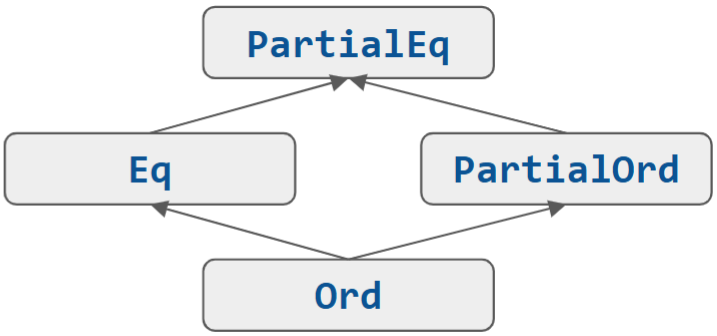
\includegraphics[width=\linewidth]{content/API_Programming/images/2026-03-24-15-45-17.png}
  \end{minipage}
\end{flushleft}

\section{Visualizzare i contenuti}

Il tratto \textbf{Display} crea una visualizzazionecomprensibile ad un utente fianle.
Questo tratto deve essere implementato manualmente e da un punto di vista pratico,
la sua implementazione richiede la definizione di un solo metodo.

\begin{minted}[breaklines]{rust}
        trait Display {
          fn fmt(&self, f: &mut fmt::Formatter<'_>) -> fmt::Result;
        }
\end{minted}

Il tratto \textbf{Debug} ha la stessa firma di \textbf{Dispaly}. Il suo scopo,
tuttavia, è differente: creare una rappresentazione comprensibile al
programmatore del valore.

\begin{itemize}
  \item Viene attivato usando il segnaposto \verb|{:?}| nelle macro di stampa
  \item Può essere sintetizzato automaticamente attraverso l'annotazione \verb|#[derive(Debug)]|
\end{itemize}

\section{Copia e duplicazione}

\subsection{Clone}

Il tratto \textbf{Clone} indica la capacità di un tipo di creare un duplicato di un
valore dato.
Può essere usato per trasformare un riferimento, \textbf{\&T} in un valore
posseduto, \textbf{T}.

Tale trasformazione, ovviamente, può essere molto costosa in termini di tempo e
memoria, tuttavia è sempre sotto il controllo del programmatore perché tale
funzionalità non è mai attivata automaticamente.

\subsection{Copy}

Il tratto \textbf{Copy} è un sotto-tratto di \textbf{Clone}.

\begin{itemize}
  \item Esso implica il fatto che la copia ottenuta sia - a tutti gli effetti
        - il solo duplicato dei bit presenti nel valore originale, senza nessuna
        trasformazione

  \item La sua implementazione può essere veloce ed efficiente, infatti si basa sulla
        duplicazione bit-a-bit del valore originale

  \item La presenza del tratto \textbf{Copy} trasforma la semantica delle operazioni di assegnazione.
        Quello che normalmente determina un movimento, che rende inaccessibile il
        valore originale, diventa una copia.
\end{itemize}

\section{Rilasciare le risorse}

Il tratto \textbf{Drop} permette di definire il metodo \verb|drop(&mut self)| che fa le veci
del distruttore nel linguaggio C++.

Il compilatore Rust garantisce che tale metodo sarà chiamato nel momento in cui
la variabile che contiene un valore di questo tipo uscirà dal proprio scope
sintattico o subito prima che le venga assegnato un nuovo valore.


Questo permette di rilasciare eventuali risorse possedute dalla struttura dati o
abilitare comportamenti duali a quelli della creazione dell'oggetto, tipici del
pattern \textit{RAII - Resource Acquisition Is Initialization}.

Questo tratto è mutuamente esclusivo con il tratto \textbf{Copy}. Questo vincolo
elimina, in assenza di blocchi \verb|unsafe \{ ... \}|, la possibilità di avere un
doppio rilascio delle risorse presenti sullo heap.

Questo tratto si accompagna alla funzione globale \mintinline{rust}|fn drop<T>(_x:T) {}|.
Essa forza il passaggio di possesso di un valore ad una nuova variabile (\_x)
che uscirà di scena subito, provocandone la distruzione.

\section{Conversione tra tipi}
I tratti \textbf{From} e \textbf{Into} permettono di effettuare conversioni di tipo, prendono
possesso del valore lo convertono e ritornano il possesso al chiamante.


I tratti sono perfettamente duali, scrivere \mintinline{rust}|T: From<i32>| equivale a scrivere \mintinline{rust}|i32: Into<T>|.

Se si implementa \textbf{From}, il tratto \textbf{Into} viene generato automaticamente.

L'implementazione del tratto \textbf{From NON È SIMMETRICA}: se è possibile passare
dal tipo \textbf{T} al tipo \textbf{U}, non è affatto detto che sia possibile
tornare indietro, da \textbf{U} a \textbf{T}.

\begin{minted}[breaklines]{rust}
trait From<T>: Sized {
  fn from(other: T) -> Self;
}

trait Into<T>: Sized {
  fn into(self) -> T;
}
\end{minted}

Il tratto \textbf{FromStr} permette di gestire la conversione da stringa e l'eventuale
fallimento. Il metodo \mintinline{rust}|from_str()| viene implicitamente richiamato
tutte le volte che si utilizza il metodo \mintinline{rust}|parse|

\begin{minted}[breaklines]{rust}
pub trait FromStr{
  type Err;
  fn from_str(s: &str) -> Result<Self, Self::Err>;
}
\end{minted}






